\documentclass[journal,12pt,twocolumn]{IEEEtran}

\usepackage{setspace}
\usepackage{gensymb}
\singlespacing
\usepackage[cmex10]{amsmath}

\usepackage{amsthm}

\usepackage{mathrsfs}
\usepackage{txfonts}
\usepackage{stfloats}
\usepackage{bm}
\usepackage{cite}
\usepackage{cases}
\usepackage{subfig}

\usepackage{longtable}
\usepackage{multirow}

\usepackage{enumitem}
\usepackage{mathtools}
\usepackage{steinmetz}
\usepackage{tikz}
\usepackage{circuitikz}
\usepackage{verbatim}
\usepackage{tfrupee}
\usepackage[breaklinks=true]{hyperref}
\usepackage{graphicx}
\usepackage{tkz-euclide}

\usetikzlibrary{calc,math}
\usepackage{listings}
    \usepackage{color}                                            %%
    \usepackage{array}                                            %%
    \usepackage{longtable}                                        %%
    \usepackage{calc}                                             %%
    \usepackage{multirow}                                         %%
    \usepackage{hhline}                                           %%
    \usepackage{ifthen}                                           %%
    \usepackage{lscape}     
\usepackage{multicol}
\usepackage{chngcntr}

\DeclareMathOperator*{\Res}{Res}

\renewcommand\thesection{\arabic{section}}
\renewcommand\thesubsection{\thesection.\arabic{subsection}}
\renewcommand\thesubsubsection{\thesubsection.\arabic{subsubsection}}

\renewcommand\thesectiondis{\arabic{section}}
\renewcommand\thesubsectiondis{\thesectiondis.\arabic{subsection}}
\renewcommand\thesubsubsectiondis{\thesubsectiondis.\arabic{subsubsection}}


\hyphenation{op-tical net-works semi-conduc-tor}
\def\inputGnumericTable{}                                 %%

\lstset{
%language=C,
frame=single, 
breaklines=true,
columns=fullflexible
}
\begin{document}


\newtheorem{theorem}{Theorem}[section]
\newtheorem{problem}{Problem}
\newtheorem{proposition}{Proposition}[section]
\newtheorem{lemma}{Lemma}[section]
\newtheorem{corollary}[theorem]{Corollary}
\newtheorem{example}{Example}[section]
\newtheorem{definition}[problem]{Definition}

\newcommand{\BEQA}{\begin{eqnarray}}
\newcommand{\EEQA}{\end{eqnarray}}
\newcommand{\define}{\stackrel{\triangle}{=}}
\bibliographystyle{IEEEtran}
\raggedbottom
\setlength{\parindent}{0pt}
\providecommand{\mbf}{\mathbf}
\providecommand{\pr}[1]{\ensuremath{\Pr\left(#1\right)}}
\providecommand{\qfunc}[1]{\ensuremath{Q\left(#1\right)}}
\providecommand{\sbrak}[1]{\ensuremath{{}\left[#1\right]}}
\providecommand{\lsbrak}[1]{\ensuremath{{}\left[#1\right.}}
\providecommand{\rsbrak}[1]{\ensuremath{{}\left.#1\right]}}
\providecommand{\brak}[1]{\ensuremath{\left(#1\right)}}
\providecommand{\lbrak}[1]{\ensuremath{\left(#1\right.}}
\providecommand{\rbrak}[1]{\ensuremath{\left.#1\right)}}
\providecommand{\cbrak}[1]{\ensuremath{\left\{#1\right\}}}
\providecommand{\lcbrak}[1]{\ensuremath{\left\{#1\right.}}
\providecommand{\rcbrak}[1]{\ensuremath{\left.#1\right\}}}
\theoremstyle{remark}
\newtheorem{rem}{Remark}
\newcommand{\sgn}{\mathop{\mathrm{sgn}}}
\providecommand{\abs}[1]{\left\vert#1\right\vert}
\providecommand{\res}[1]{\Res\displaylimits_{#1}} 
\providecommand{\norm}[1]{\left\lVert#1\right\rVert}
%\providecommand{\norm}[1]{\lVert#1\rVert}
\providecommand{\mtx}[1]{\mathbf{#1}}
\providecommand{\mean}[1]{E\left[ #1 \right]}
\providecommand{\fourier}{\overset{\mathcal{F}}{ \rightleftharpoons}}
%\providecommand{\hilbert}{\overset{\mathcal{H}}{ \rightleftharpoons}}
\providecommand{\system}{\overset{\mathcal{H}}{ \longleftrightarrow}}
	%\newcommand{\solution}[2]{\textbf{Solution:}{#1}}
\newcommand{\solution}{\noindent \textbf{Solution: }}
\newcommand{\cosec}{\,\text{cosec}\,}
\providecommand{\dec}[2]{\ensuremath{\overset{#1}{\underset{#2}{\gtrless}}}}
\newcommand{\myvec}[1]{\ensuremath{\begin{pmatrix}#1\end{pmatrix}}}
\newcommand{\mydet}[1]{\ensuremath{\begin{vmatrix}#1\end{vmatrix}}}
\numberwithin{equation}{subsection}
\makeatletter
\@addtoreset{figure}{problem}
\makeatother
\let\StandardTheFigure\thefigure
\let\vec\mathbf
\renewcommand{\thefigure}{\theproblem}
\def\putbox#1#2#3{\makebox[0in][l]{\makebox[#1][l]{}\raisebox{\baselineskip}[0in][0in]{\raisebox{#2}[0in][0in]{#3}}}}
     \def\rightbox#1{\makebox[0in][r]{#1}}
     \def\centbox#1{\makebox[0in]{#1}}
     \def\topbox#1{\raisebox{-\baselineskip}[0in][0in]{#1}}
     \def\midbox#1{\raisebox{-0.5\baselineskip}[0in][0in]{#1}}
\vspace{3cm}
\title{Assignment-1}
\author{Ganraj Borade - EE18BTECH11016}
\maketitle
\newpage
\bigskip
\renewcommand{\thefigure}{\theenumi}
\renewcommand{\thetable}{\theenumi}
Download all python codes from 
\begin{lstlisting}
https://github.com/ganrajborade/EE3025/tree/main/A1/codes
\end{lstlisting}
%
and latex-tikz codes from 
%
\begin{lstlisting}
https://github.com/ganrajborade/EE3025/tree/main/A1
\end{lstlisting}

\section{Problem}
\begin{enumerate}[label=\thesection.\arabic*.,ref=\thesection.\theenumi]
    \numberwithin{equation}{enumi}
    
    \item Let
    \begin{align}
        x(n) = \cbrak{\underset{\uparrow}{1},2,3,4,2,1}
         \label{eq:equation0}\\
        y(n) + \frac{1}{2}y(n-1) = x(n) + x(n-2)	
        \label{eq:equation1}
    \end{align}
    
    \item Compute 
    \begin{align}
        X(k) \triangleq \sum_{n=0}^{N-1} x(n) e^{-j 2 \pi k n / N}, \quad k=0,1, \ldots, N-1
    \end{align}
    and $H(k)$ using h(n).
    
    \item Compute 
    \begin{align}
    Y(k) = X(k)H(k)
    \end{align}
\end{enumerate}

\section{Solution}
\begin{enumerate}[label=\thesection.\arabic*.,ref=\thesection.\theenumi]
\numberwithin{equation}{enumi}
\item
The Impulse Response of the LTI system is the output of the system when Unit Impulse Signal is given as input to the system.
Impulse response h(n) can be found from given difference equation as follows (h(n) is IIR Filter)
\begin{align}
    h(n) + \frac{1}{2}h(n-1) = \delta(n) + \delta(n-2)	
    \label{eq:equation4}
\end{align}

\item
DFT of a Input Signal $x(n)$ is 
\begin{align}
X(k) \triangleq \sum_{n=0}^{N-1} x(n) e^{-j 2 \pi k n / N}, \quad k=0,1, \ldots, N-1
\end{align}

\item
Let $W_{N} = e^{-j2\pi/N} \\$ 
We can express X as Matrix Multiplication of DFT Matrix and x.
\begin{equation}
X = 
\begin{bmatrix}
W^{ij}_{N} 
\end{bmatrix}_{N \times N}
x, \quad i,j = 0,1, \ldots, N-1
\end{equation}





\item
Using the property of complex exponentials :
\begin{align}
	 W^{2}_{N} =  W_{N/2}  
\end{align}

\begin{align}
\mathcal X(k) &=  \sum_{n=0}^{N-1} x(n)W^{kn}_{N}, \quad k=0,1, \ldots, N-1 \\
&= \sum_{n=even} x(n)W^{kn}_{N} + \sum_{n=odd} x(n)W^{kn}_{N} \\
&= \sum_{m=0}^{2} x(2m)W^{2mk}_{N} + \sum_{m=0}^{2} x(2m+1)W^{(2m+1)k}_{N} 
\end{align}
using property above property, we get,
\begin{align}
\mathcal X(k) &= \sum_{m=0}^{2} x(2m)W^{mk}_{N/2} + W^{k}_{N} \sum_{m=0}^{2} x(2m+1)W^{mk}_{N/2} \\
&= X_{1}(k) + W^{k}_{N}X_{2}(k)
\end{align}

\begin{itemize}
	\item Here,X\textsubscript{1}(k) and X\textsubscript{2}(k) are 3 point DFTs of x(2m) and x(2m+1) , m=0,1,2.
	\item And X\textsubscript{1}(k) and X\textsubscript{2}(k) are periodic, Hence X\textsubscript{1}(k+3) = X\textsubscript{1}(k) and X\textsubscript{2}(k+3) = X\textsubscript{1}(k).
\end{itemize}

\item Calculating X1 and X2
\begin{align}
X_{1}(k) = \sum_{m=0}^{2} x(2m)W^{mk}_{3} \\
X_{2}(k) = \sum_{m=0}^{2} x(2m+1)W^{mk}_{3}
\end{align}

\begin{equation}
\begin{bmatrix}
X_{1}(0) \\ 
X_{1}(1) \\ 
X_{1}(2) \\ 
X_{2}(0) \\ 
X_{2}(1) \\ 
X_{2}(2)
\end{bmatrix}
=
\begin{bmatrix}
W^{0}_{3} & W^{0}_{3} & W^{0}_{3} & 0 & 0 & 0\\
W^{0}_{3} & W^{1}_{3} & W^{2}_{3} & 0 & 0 & 0\\
W^{0}_{3} & W^{2}_{3} & W^{4}_{3} & 0 & 0 & 0\\
0 & 0 & 0 & W^{0}_{3} & W^{0}_{3} & W^{0}_{3}\\
0 & 0 & 0 & W^{0}_{3} & W^{1}_{3} & W^{2}_{3}\\
0 & 0 & 0 & W^{0}_{3} & W^{2}_{3} & W^{4}_{3}
\end{bmatrix}
\begin{bmatrix}
x(0) \\ 
x(2) \\ 
x(4) \\ 
x(1) \\ 
x(3) \\ 
x(5) 
\end{bmatrix}   
\end{equation}

\item Calculating X
\begin{align}
X(k) = X_{1}(k) + W^{k}_{N}X_{2}(k)
\end{align}

\begin{equation}
\begin{bmatrix}
X(0) \\ 
X(1) \\ 
X(2) \\ 
X(3) \\ 
X(4) \\ 
X(5) 
\end{bmatrix}
=
\begin{bmatrix}
1 & 0 & 0 & W^{0}_{6} & 0 & 0\\
0 & 1 & 0 &  0 & W^{1}_{6} & 0\\
0 & 0 & 1 & 0 & 0 & W^{2}_{6}\\
1 & 0 & 0 & W^{3}_{6} & 0 & 0\\
0 & 1 & 0 & 0 & W^{4}_{6} & 0\\
0 & 0 & 1 & 0 & 0 & W^{5}_{6}
\end{bmatrix}
\begin{bmatrix}
X_{1}(0) \\ 
X_{1}(1) \\ 
X_{1}(2) \\ 
X_{2}(0) \\ 
X_{2}(1) \\ 
X_{2}(2)
\end{bmatrix}
\label{eq:equation8}
\end{equation}
\begin{equation}
\implies
\begin{bmatrix} 
X(0) \\ 
X(1) \\ 
X(2) \\ 
X(3) \\ 
X(4) \\ 
X(5) 
\end{bmatrix}
=
\begin{bmatrix}
13+0j \\ 
-4-\sqrt{3}j\\ 
1+0j \\ 
-1+0j\\ 
1+0j \\ 
-4+\sqrt{3}j
\end{bmatrix}
\end{equation}








\item

DFT of a Impulse Response $h(n)$ is 
\begin{align}
H(k) \triangleq \sum_{n=0}^{N-1} h(n) e^{-j 2 \pi k n / N}, \quad k=0,1, \ldots, N-1
\end{align}
\item
Now to find $H(k)$ we need to know h(n) first. So we will first calculate h(n). For that we need to first find the H(z) by applying Z-transform on equation $\eqref{eq:equation4}$ i.e.,

\begin{align}
H(z) = \frac{2(z^2+1)}{z(2z+1)}
\end{align}
\begin{align}
H(z) = \frac{1+z^{-2}}{1+\frac{1}{2}z^{-1}}
\end{align}
From this we can say that h(n) is,
\begin{align}
h(n)= Z^{-1}\sbrak{\frac{1}{1+\frac{1}{2}z^{-1}} + \frac{z^{-2}}{1+\frac{1}{2}z^{-1}}}
\end{align}
\begin{align}
h(n)=\sbrak{\frac{-1}{2}}^nu(n) + \sbrak{\frac{-1}{2}}^{n-2}u(n-2)
\end{align}
Similarly, like X(k), we can calculate H(k).

\begin{align}
W_{1} = 
\begin{bmatrix}
	1 & 0 & 0 & W^{0}_{6} & 0 & 0\\
	0 & 1 & 0 &  0 & W^{1}_{6} & 0\\
	0 & 0 & 1 & 0 & 0 & W^{2}_{6}\\
	1 & 0 & 0 & W^{3}_{6} & 0 & 0\\
	0 & 1 & 0 & 0 & W^{4}_{6} & 0\\
	0 & 0 & 1 & 0 & 0 & W^{5}_{6}
\end{bmatrix}
\end{align}



\begin{align}
W_{2} = 
\begin{bmatrix}
W^{0}_{3} & W^{0}_{3} & W^{0}_{3} & 0 & 0 & 0\\
W^{0}_{3} & W^{1}_{3} & W^{2}_{3} & 0 & 0 & 0\\
W^{0}_{3} & W^{2}_{3} & W^{4}_{3} & 0 & 0 & 0\\
0 & 0 & 0 & W^{0}_{3} & W^{0}_{3} & W^{0}_{3}\\
0 & 0 & 0 & W^{0}_{3} & W^{1}_{3} & W^{2}_{3}\\
0 & 0 & 0 & W^{0}_{3} & W^{2}_{3} & W^{4}_{3}
\end{bmatrix}
\end{align}
Same as we done while calculating X(k) using Eq \eqref{eq:equation8}
\begin{equation}
\begin{bmatrix} 
H(0) \\ 
H(1) \\ 
H(2) \\ 
H(3) \\ 
H(4) \\ 
H(5) 
\end{bmatrix}
=
W_{1}W_{2}
\begin{bmatrix}
h(0) \\ 
h(2) \\ 
h(4) \\ 
h(1) \\ 
h(3) \\ 
h(5)
\end{bmatrix}
\end{equation}


\begin{equation}
\implies
\begin{bmatrix} 
H(0) \\ 
H(1) \\ 
H(2) \\ 
H(3) \\ 
H(4) \\ 
H(5) 
\end{bmatrix}
=
\begin{bmatrix}
1.28125+0j \\
0.51625-0.5142j \\ 
-0.07813+1.1096j  \\ 
3.84375+0j \\ 
-0.07183-1.1096j \\ 
0.51625+0.5142j
\end{bmatrix}
\end{equation}


\item We can now compute $Y(k)$ using 	Eq \eqref{eq:equation2}
\begin{align}
Y(k) = X(k)H(k)
\label{eq:equation2}
\end{align}
So, $Y(k)$ is obtained element wise multiplication of $X(k)$ and $H(k)$
\begin{equation}
\renewcommand{\arraystretch}{1.45}
\setlength\arraycolsep{0.01pt}
\begin{bmatrix} 
Y(0) \\ Y(1) \\ Y(2) \\ Y(3) \\ Y(4) \\ Y(5) 
\end{bmatrix}
=
\begin{bmatrix}
X(0)\cdot H(0) \\ X(1)\cdot H(1) \\ X(2)\cdot H(2) \\ X(3)\cdot H(3) \\ X(4)\cdot H(4) \\ X(5)\cdot H(5)
\end{bmatrix}
\end{equation}
Computing the above expression we get,
\begin{equation}
\renewcommand{\arraystretch}{1.45}
\setlength\arraycolsep{0.01pt}
\begin{bmatrix} 
Y(0) \\ Y(1) \\ Y(2) \\ Y(3) \\ Y(4) \\ Y(5) 
\end{bmatrix}
=
\begin{bmatrix}
16.6562+0j \\ -2.95312+1.16372j \\ -0.07812+1.10959j \\ -3.84375-9.27556j \\ -0.07812-1.10959j \\ -2.95312-1.16372j 
\end{bmatrix}
\end{equation}

\item The following code computes Y and generates magnitude and phase plots of X, H, Y
\begin{lstlisting}
https://github.com/ganrajborade/EE3025/blob/main/A1/codes/EE18BTECH11016.py
\end{lstlisting}

\item The following plots are obtained
\begin{figure}[!ht]
	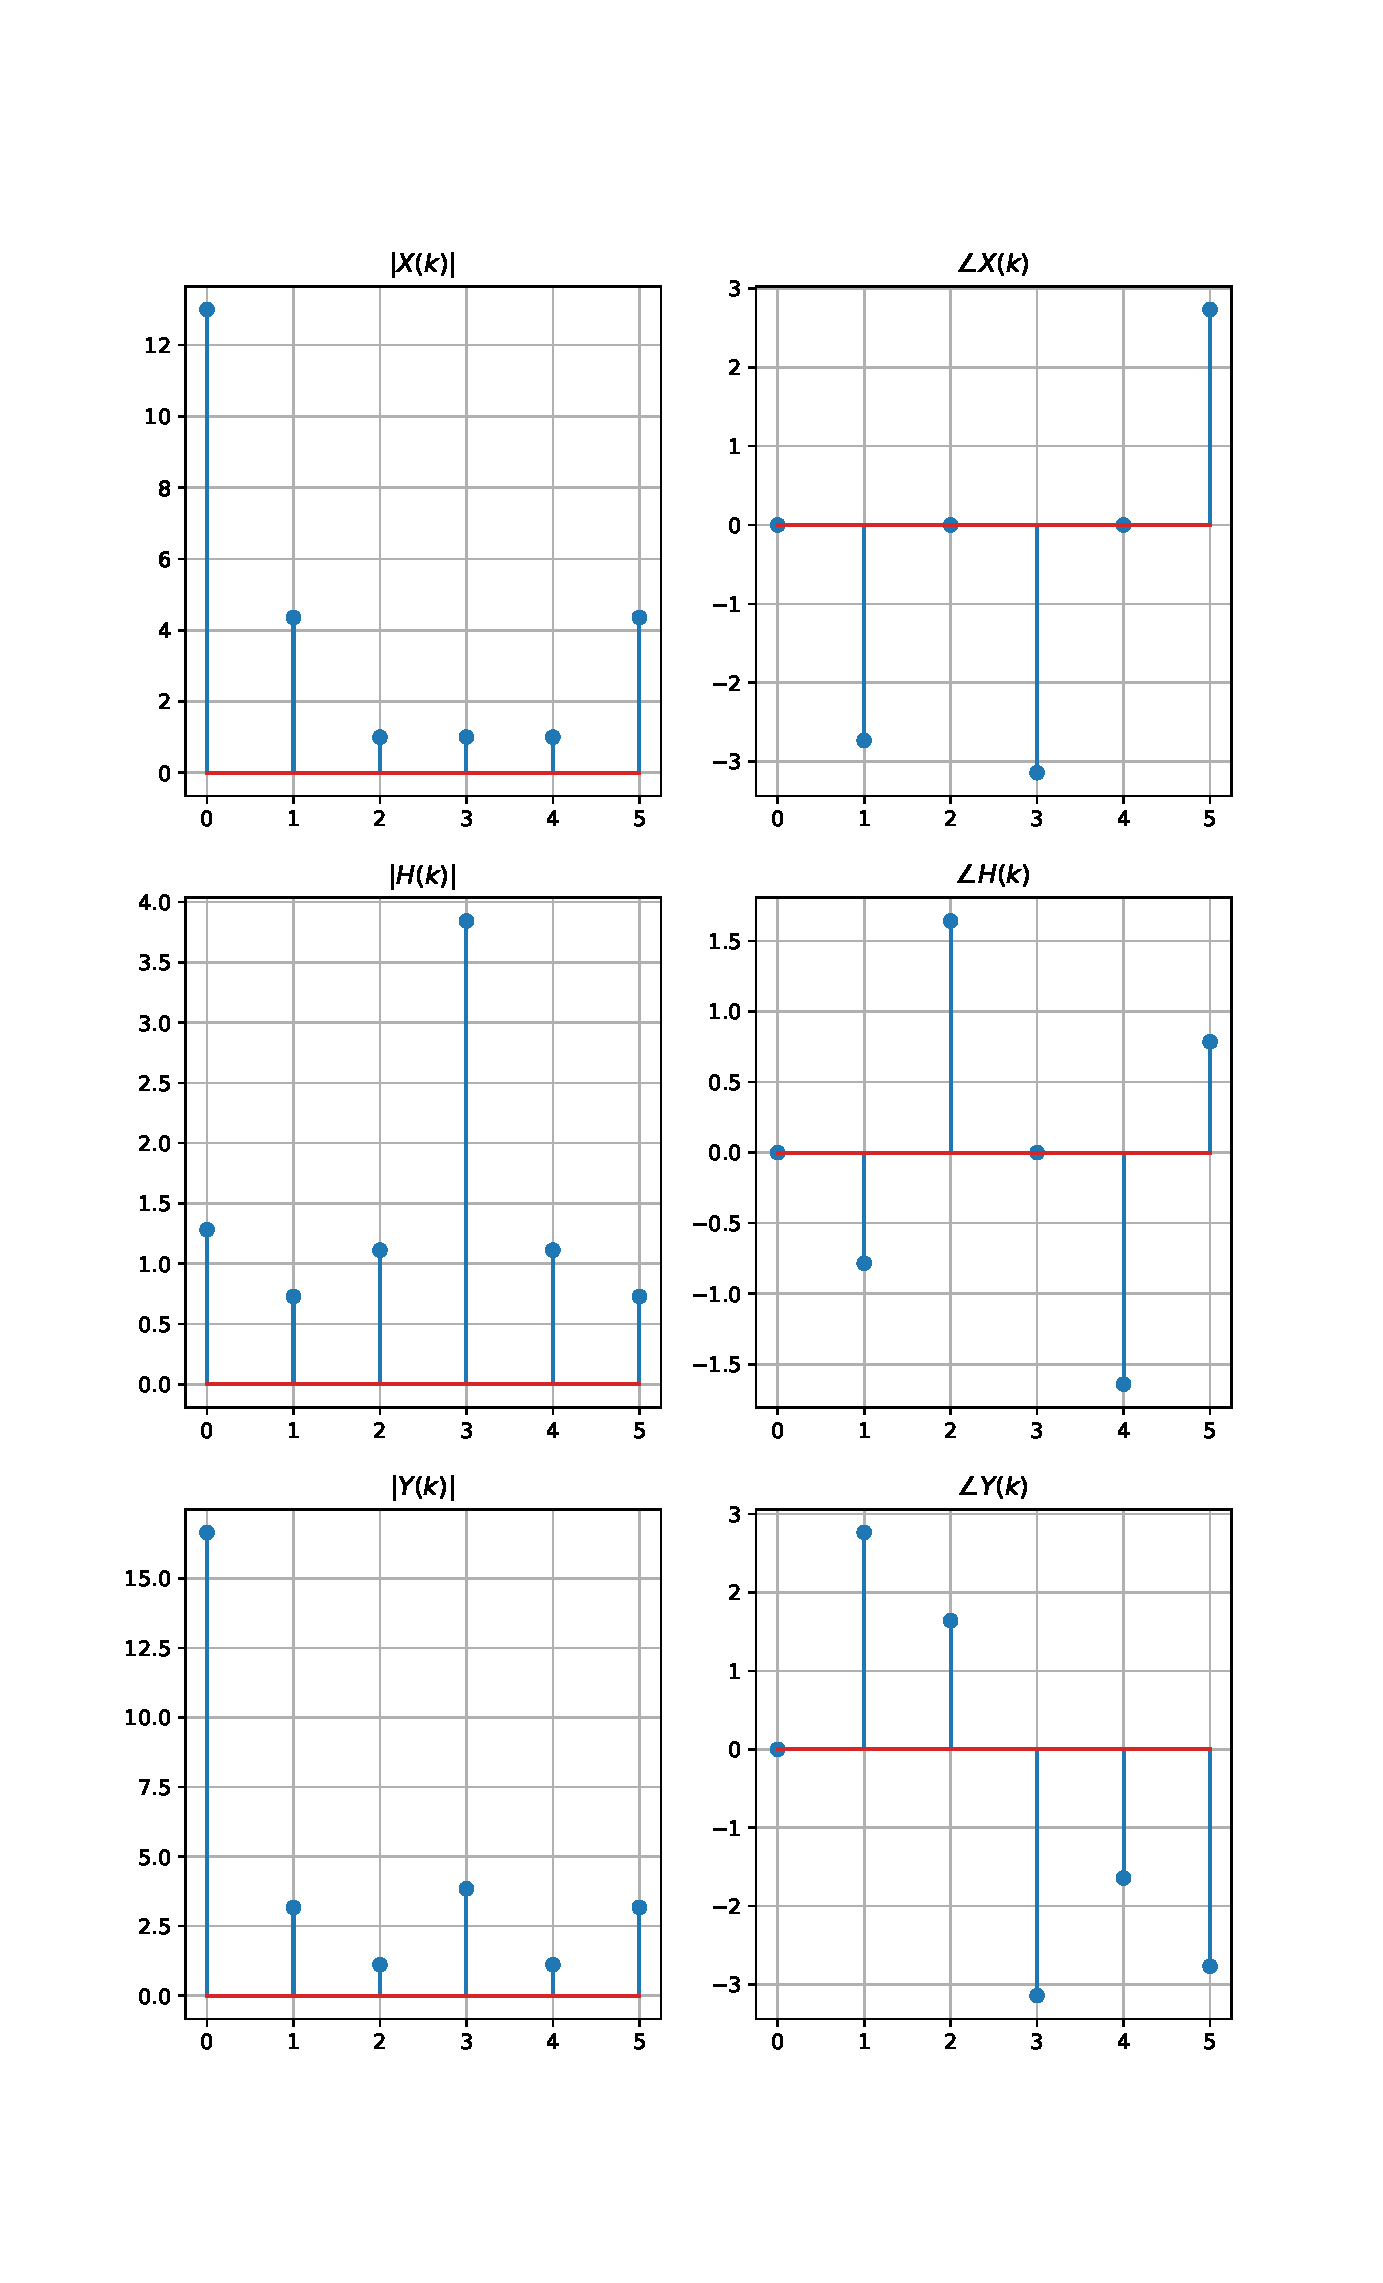
\includegraphics[width=9.5cm]{./figs/EE18BTECH11016.eps}
\end{figure}
\end{enumerate}
\end{document}
